\documentclass{beamer}

\usepackage{fontspec,xunicode,xltxtra}

\usepackage{tikz}

\XeTeXlinebreaklocale "zh"
\XeTeXlinebreakskip = 0pt plus 1pt minus 0.1pt

%\setmainfont[Mapping=tex-text]{AR PL UMing CN:style=Light}
%\setmainfont[Mapping=tex-text]{AR PL UKai CN:style=Book}
%\setmainfont[Mapping=tex-text]{WenQuanYi Zen Hei:style=Regular}
%\setmainfont[Mapping=tex-text]{WenQuanYi Zen Hei Sharp:style=Regular}
%\setmainfont[Mapping=tex-text]{AR PL KaitiM GB:style=Regular} 
%\setmainfont[Mapping=tex-text]{AR PL SungtiL GB:style=Regular} 
%\setmainfont[Mapping=tex-text]{WenQuanYi Zen Hei Mono:style=Regular} 


\newfontfamily\hei{WenQuanYi Micro Hei}
\newfontfamily\whei{WenQuanYi Zen Hei}
\newfontfamily\kai{AR PL UKai CN}
\newfontfamily\song{AR PL UMing CN}
\newfontfamily\bhei{cwTeXHeiBold}
%\newfontfamily\lishu{SIMLI}
\setmainfont[Mapping=tex-text]{WenQuanYi Micro Hei}
\setsansfont[Mapping=tex-text]{AR PL UKai CN}
\setmonofont[Mapping=tex-text]{WenQuanYi Zen Hei Mono}

\renewcommand{\baselinestretch}{1.25}


\mode<presentation>
{
  \usetheme{Darmstadt}

 % \usetheme{Warsaw}
  % or ...
%  \usetheme{default}

  \setbeamercovered{transparent}
  % or whatever (possibly just delete it)
}


\usepackage[english]{babel}
% or whatever

%\usepackage[latin1]{inputenc}
% or whatever

\title[Beamer + xelatex] % (optional, use only with long paper titles)
{\Huge 数学软件: 数学工作者应该如何使用计算机}

\subtitle
{专题一:环境和习惯} % (optional)

\author[Wang HY] % (optional, use only with lots of authors)
{王何宇}
% - Use the \inst{?} command only if the authors have different
%   affiliation.

\institute[ZJU] % (optional, but mostly needed)
{
  浙江大学数学科学学院\\
  信息与计算科学系
}
% - Use the \inst command only if there are several affiliations.
% - Keep it simple, no one is interested in your street address.

\date[] % (optional)
{}


% If you have a file called "university-logo-filename.xxx", where xxx
% is a graphic format that can be processed by latex or pdflatex,
% resp., then you can add a logo as follows:

\pgfdeclareimage[height=1cm]{university-logo}{../images/zju.jpg}
\logo{\pgfuseimage{university-logo}}

% Delete this, if you do not want the table of contents to pop up at
% the beginning of each subsection:
%\AtBeginSubsection[]
%{
%  \begin{frame}<beamer>{Outline}
%    \tableofcontents[currentsection,currentsubsection]
%  \end{frame}
%}


% If you wish to uncover everything in a step-wise fashion, uncomment
% the following command: 

%\beamerdefaultoverlayspecification{<+->}


\begin{document}

\begin{frame}
 \titlepage
\end{frame}

% \begin{frame}{提纲}
%   \tableofcontents
%   % You might wish to add the option [pausesections]
% \end{frame}

\begin{frame}{自我介绍}
  \begin{itemize}
  \item 王何宇, 浙江大学数学科学学院, 信息与计算科学系.
  \item email: wangheyu@zju.edu.cn
  \item 手机: 13456940632
  \item 我承担很多信息与计算方向的专业课程, 所以大概率会和大家共事 3 年甚至更多.
  \end{itemize}
\end{frame}

\begin{frame}{本课主要内容}
  \begin{itemize}
  \item<1-> 数学院实践环节课程,名字有点过时了,暂时懒得改。
  \item<2-> 使用计算机从事数学学习和科研。
  \item<3-> 主要内容:
    \begin{itemize}
    \item<3-> AI 工具的使用.
    \item<3-> 搭建数学工作环境.
    \item<3-> 培养现代化的数学工作习惯.
    \item<3-> 常用数学软件介绍.
    \item<3-> 综合上述技能完成一些数学建模和科研任务.
    \end{itemize}
  \item<4-> 本课程是为数学院学生定制的,非相关专业同学慎选!
  \end{itemize}
\end{frame}

% \begin{frame}{工作环境的剧烈变化}
%   \begin{itemize}
%   \item<1-> 从纸笔到黑板,再到计算机,现在是 AI,特别是大语言模型.
%   \item<2-> 我们是否应该在数学学习和科研中全面接受大语言模型?
%   \item<3-> 这不是应不应该,而是已经发生的事实:几乎人人都在用!
%   \item<4-> AI 工具的实际意义:提高工作效率,提高工作质量,特别是在非数学环节。此外还要考虑 AI 在迅速进步。
%   \item<5-> 一些中古的技能也应掌握:\LaTeX, 编辑器,编程,shell, git, ... 
%   \end{itemize}
% \end{frame}

\begin{frame}{个人案例:如何阅读一篇数学论文}
  \begin{columns}[t]
  \begin{column}{.5\textwidth}
  \begin{itemize}
  \item<1-> 科研和学习的起点是选择文献. 
  \item<2-> 如何精度一篇论文(\hei{相当个人})\cite{robbins1951stochastic}。
  \item<3-> 和大模型进行数学讨论。
  \item<4-> 模拟和验证论文的结果。
  \item<5-> 总结和记录讨论的内容。
  \end{itemize}
\end{column}
\begin{column}{.5\textwidth}
  \begin{figure}
    \centering
    \includegraphics<1>[width=0.75\textwidth]{../images/ruby_paper.PNG}
    \includegraphics<2>[width=0.75\textwidth]{../images/good_paper.PNG}
    \includegraphics<3>[width=0.75\textwidth]{../images/Aidiot.PNG}
    \includegraphics<4>[width=0.75\textwidth]{../images/sgd.PNG}
    \includegraphics<5>[width=0.75\textwidth]{../images/report.PNG}
  \end{figure}
\end{column}
\end{columns}
\end{frame}

% \begin{frame}{工作环境介绍}
%   \begin{itemize}
%   \item<1-> 大模型的选择:GPT*, Qianwen, Deepseek(有校内版), kimi, 综合平台, ...
%   \item<2-> 操作系统:Windows 11 + wsl 2, 事实上不重要,需要一个 linux 终端环境.
%   \item<3-> 编辑器:vscode.
%   \item<4-> 项目管理:git. 平台:github, gitee, zjugit, ...
%   \end{itemize}
% \end{frame}


% \begin{frame}{工作环境介绍}
%   \begin{columns}[c]
% % create the column with the first image, that occupies
% % half of the slide
%     \begin{column}{.5\textwidth}
%       \begin{itemize}
%       \item<1-> 繁华下的真像: 二进制流. 
%       \item<2-> 控制计算机, 而不是被控制.
%       \item<3-> core 归计算机, shell 归愚蠢的人类.
%       \item<4-> 掌握了 Terminal/shell, 才能真正掌握计算机(才怪).
%       \end{itemize}
%     \end{column}
% % create the column with the second image, that also
% % occupies half of the slide
%     \begin{column}{.5\textwidth}
%     \begin{figure}
%         \centering
%         \includegraphics<1->[width=0.75\textwidth]{../images/matrix.bmp}
%         \includegraphics<2->[width=0.75\textwidth]{../images/matrixbin.png}
%     \end{figure}
%     \end{column}
% \end{columns}
%   %% \begin{tikzpicture}
%   %%   \node (img1) {\includegraphics[height=3cm]{res/matrix.bmp}};
%   %% \end{tikzpicture}
% \end{frame}

% \begin{frame}{文本编辑器}
%   \begin{itemize}
%   \item<1-> 能基本上完全用键盘控制.
%   \item<2-> 适合终端和 shell 的模式, 不占用太多的软硬件和通讯资源.
%   \item<3-> 能快速高效地发送和接受指令, 完成编码.
%   \item<4-> 推荐: emacs, vim, vscode.
%   \item<5-> 选择一款最适合你自己, 能把你的工作效率提到最高的编辑器.
%   \item<6-> 如果你还是新手, 请盲从大佬.
%   \item<7-> 切记一切以效率为中心, 不要对编辑器提太多不切实际的要求.
%   \item<8-> 如果你不知道怎么配置你的编辑器, 用缺省配置, 或者像同行要一个配置文件. 
%   \end{itemize}
% \end{frame}

% \section{数学写作}
% \begin{frame}{如何产生漂亮的数学文章}
%   \begin{tikzpicture}[remember picture, overlay]
%     \node[left = 2cm, above = -0.1cm] at (current page.east) 
%          {
%            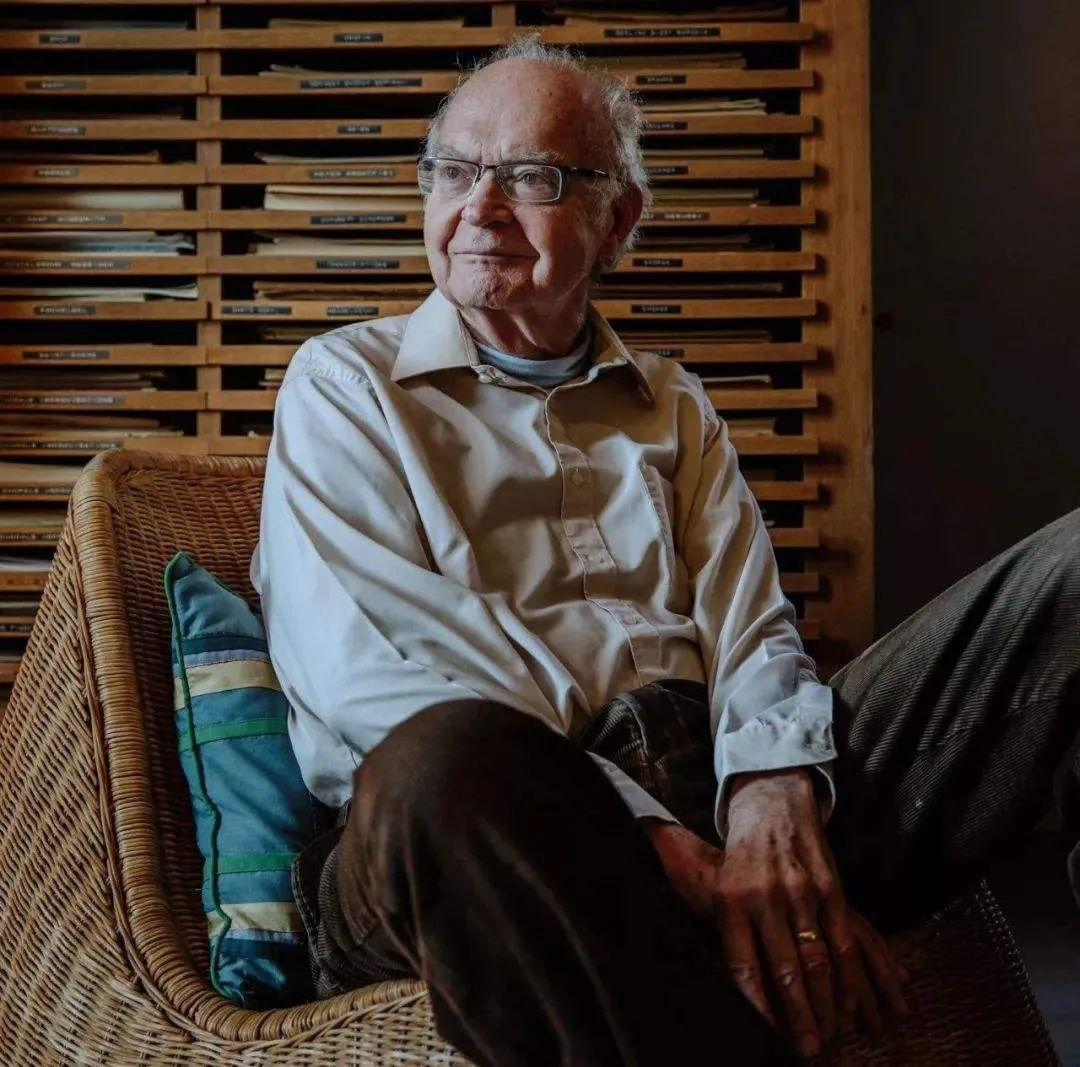
\includegraphics[width=0.25\textwidth]{../images/knuth.png}
%          };
% \end{tikzpicture}  
%   \begin{itemize}
%   \item<1-> 数学家对写作有特殊的要求.
%   \item<2-> 同样必须满足键盘, 终端和高效的原则.
%   \item<3-> 唯一解也是事实上的标准: \LaTeX.
%   \item<4-> 参考资料: lshort, manual, ...
%   \item<5-> 去找一个例子.
%   \item<6-> 必须亲自动手写点什么. 
%   \end{itemize}
% \end{frame}

% \begin{frame}{Latex进阶}
%   \begin{itemize}
%   \item<1-> 交叉引用和计数器.
%   \item<2-> 图, 表和正文混排.
%   \item<3-> 报告的制作.
%   \item<4-> 手工绘图.
%   \end{itemize}
% \end{frame}

\begin{frame}{作业:设置你的工作环境}
  \begin{itemize}
  \item<1-> 选择并熟悉你的大语言模型,可以不止一个。
  \item<2-> 准备一个 linux 环境,可以是 wsl 2, 也可以是虚拟机.
  \item<3-> 选择并安装配置一个编辑器,推荐 vscode. 
  \item<4-> 注册一个作业 git 账号,熟悉 git 的基本操作.
  \item<5-> 在作业包中两本经典教材中选择一本,根据你的兴趣选择一个主要定理的叙述和证明,加上你自己的理解,写成一份报告.
  \end{itemize}
\end{frame}

\bibliography{../mathsoft.bib}
\bibliographystyle{plain}
\end{document}


